\documentclass[9pt,twocolumn,twoside]{../../styles/osajnl}
\usepackage{fancyvrb}
\journal{i524} 

\title{KeystoneML}

\author[1,*]{Vasanth Methkupalli}

\affil[1]{School of Informatics and Computing, Bloomington, IN 47408, U.S.A.}
\affil[*]{Corresponding authors: mvasanthiiit@gmail.com}

\dates{Paper-2, \today}

\ociscodes{Cloud, I524, KeystoneML, MLlib, API, Spark}

% replace this with your url in github/gitlab
\doi{\url{https://github.com/cloudmesh/sp17-i524/blob/master/paper2/S17-IR-2019/report.pdf}}


\begin{abstract}
KeystoneML is a software framework, written in Scala, from the UC
Berkeley AMPLab designed to simplify the construction of large scale,
end-to-end, machine learning pipelines with Apache Spark. KeystoneMl
and spark.ml share many features, but however there are a few
important differences, particularly around type safety and chaining,
which lead to pipelines that are easier to construct and more
robust. KeystoneML also presents a richer set of operators than those
present in spark.ml including featurizers for images, text, and
speech, and provides several example pipelines that reproduce
state-of-the-art academic results on public data sets.
\end{abstract}

\setboolean{displaycopyright}{true}

\begin{document}

\maketitle
\TODO{This review document is provided for you to achieve your
  best. We have listed a number of obvious opportunities for
  improvement. When improving it, please keep this copy untouched and
  instead focus on improving report.tex. The review does not include
  all possible improvement suggestions and if you sea comment you may
  want to check if this comment applies elsewhere in the document.}

\section{Introduction}

MLlib’s goal is to make practical machine learning (ML) scalable and
easy. Besides new algorithms and performance improvements that are
seen in each release, a great deal of time and effort has been spent
on making MLlib easy. Similar to Spark Core, MLlib provides APIs in
three languages: Python, Java, and Scala, along with user guide and
example code, to ease the learning curve for users coming from
different backgrounds. In Apache Spark 1.2, Databricks, jointly with
AMPLab, UC Berkeley, continues this effort by introducing a pipeline
API to MLlib for easy creation and tuning of practical ML
pipelines \cite{meng2016mllib} .

A practical ML pipeline often involves a sequence of data
pre-processing, feature extraction, model fitting, and validation
stages. For example, classifying text documents might involve text
segmentation and cleaning, extracting features, and training a
classification model with cross-validation. Though there are many
libraries we can use for each stage, working with large-scale datasets
is not easy as it looks. Most ML libraries are not designed for
distributed computation or they do not provide native support for
pipeline creation and tuning. Unfortunately, this problem is often
ignored in academia, and it has received largely ad-hoc treatment in
industry, where development tends to occur in manual one-off pipeline
implementations \cite{meng2016mllib} .
\TODO{I compared with the original source. You need to first understand
the referenced documents and then state it via your own words. These
two paragraphs apparently are not "native" to this paper.}

\section{Design Principles}

KeystoneML is built on several design principles: supporting
end-to-end workflows, type safety, horizontal scalability, and
composibility. By focusing on these principles, KeystoneML allows for the
construction of complete, robust, large scale pipelines that are
constructed from reusable, understandable parts \cite{www-keystoneml1} .
\TODO{I don't think design principles deserve a dadicated section. Merge
it with intro when you update your intro section.}

\section{Key API Concepts}
At the center of KeystoneML are a handful of core API concepts that
allow us to build complex machine learning pipelines out of simple
parts:
\begin{description}

\item[$\bullet$] Pipelines
\item[$\bullet$] Nodes
\item[$\bullet$] Transformers
\item[$\bullet$] Estimators
  
 
\end{description}

\TODO{arrange the following 4 sections as sub-sections.}

\section{Pipelines}

A Pipeline is a dataflow that takes some input data and maps it to
some output data through a series of nodes. By design, these nodes can
operate on one data item (for point lookup) or many data items: for
batch model evaluation \cite{www-keystoneml1} .

In a sense, a pipeline is just a function that is composed of simpler
functions. Here’s part of the Pipeline definition:

\begin{figure}[htbp]
\centering
\fbox{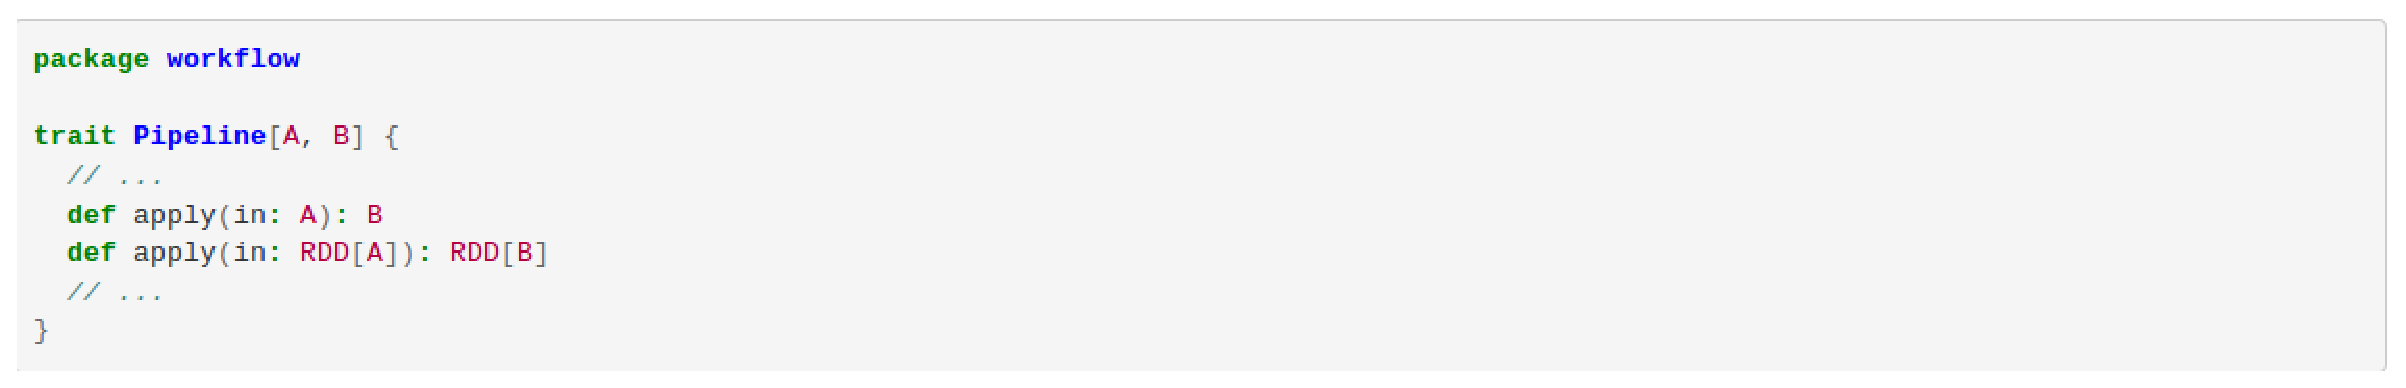
\includegraphics[width=\linewidth]{images/5}}
\caption{Pipeline Definition}
\label{fig:Pipeline Definition}
\end{figure}
\TODO{don't use fig to show code. use code style.}

From this we can see that a Pipeline has two type parameters: its
input and output types. We can also see that it has methods to operate
on just a single input data item, or on a batch RDD of data items \cite{www-keystoneml1} .

\section{Nodes}

Nodes come in two flavors:

\begin{description}
\item[$\bullet$] Transformers
\item[$\bullet$] Estimators
\end{description}

\TODO{no bullet points less than 3}

Transformers are nodes which provide a unary function interface for
both single items and RDD of the same type of item, while an Estimator
produces a Transformer based on some training data.
\subsection{Transformers}

As already mentioned, a Transformer is the simplest type of node, and
takes an input, and deterministically transforms it into an
output. Here’s an abridged definition of the Transformer class.
\TODO{where did you mention it is the simplest? some texts not pasted yet?}

\begin{figure}[htbp]
\centering
\fbox{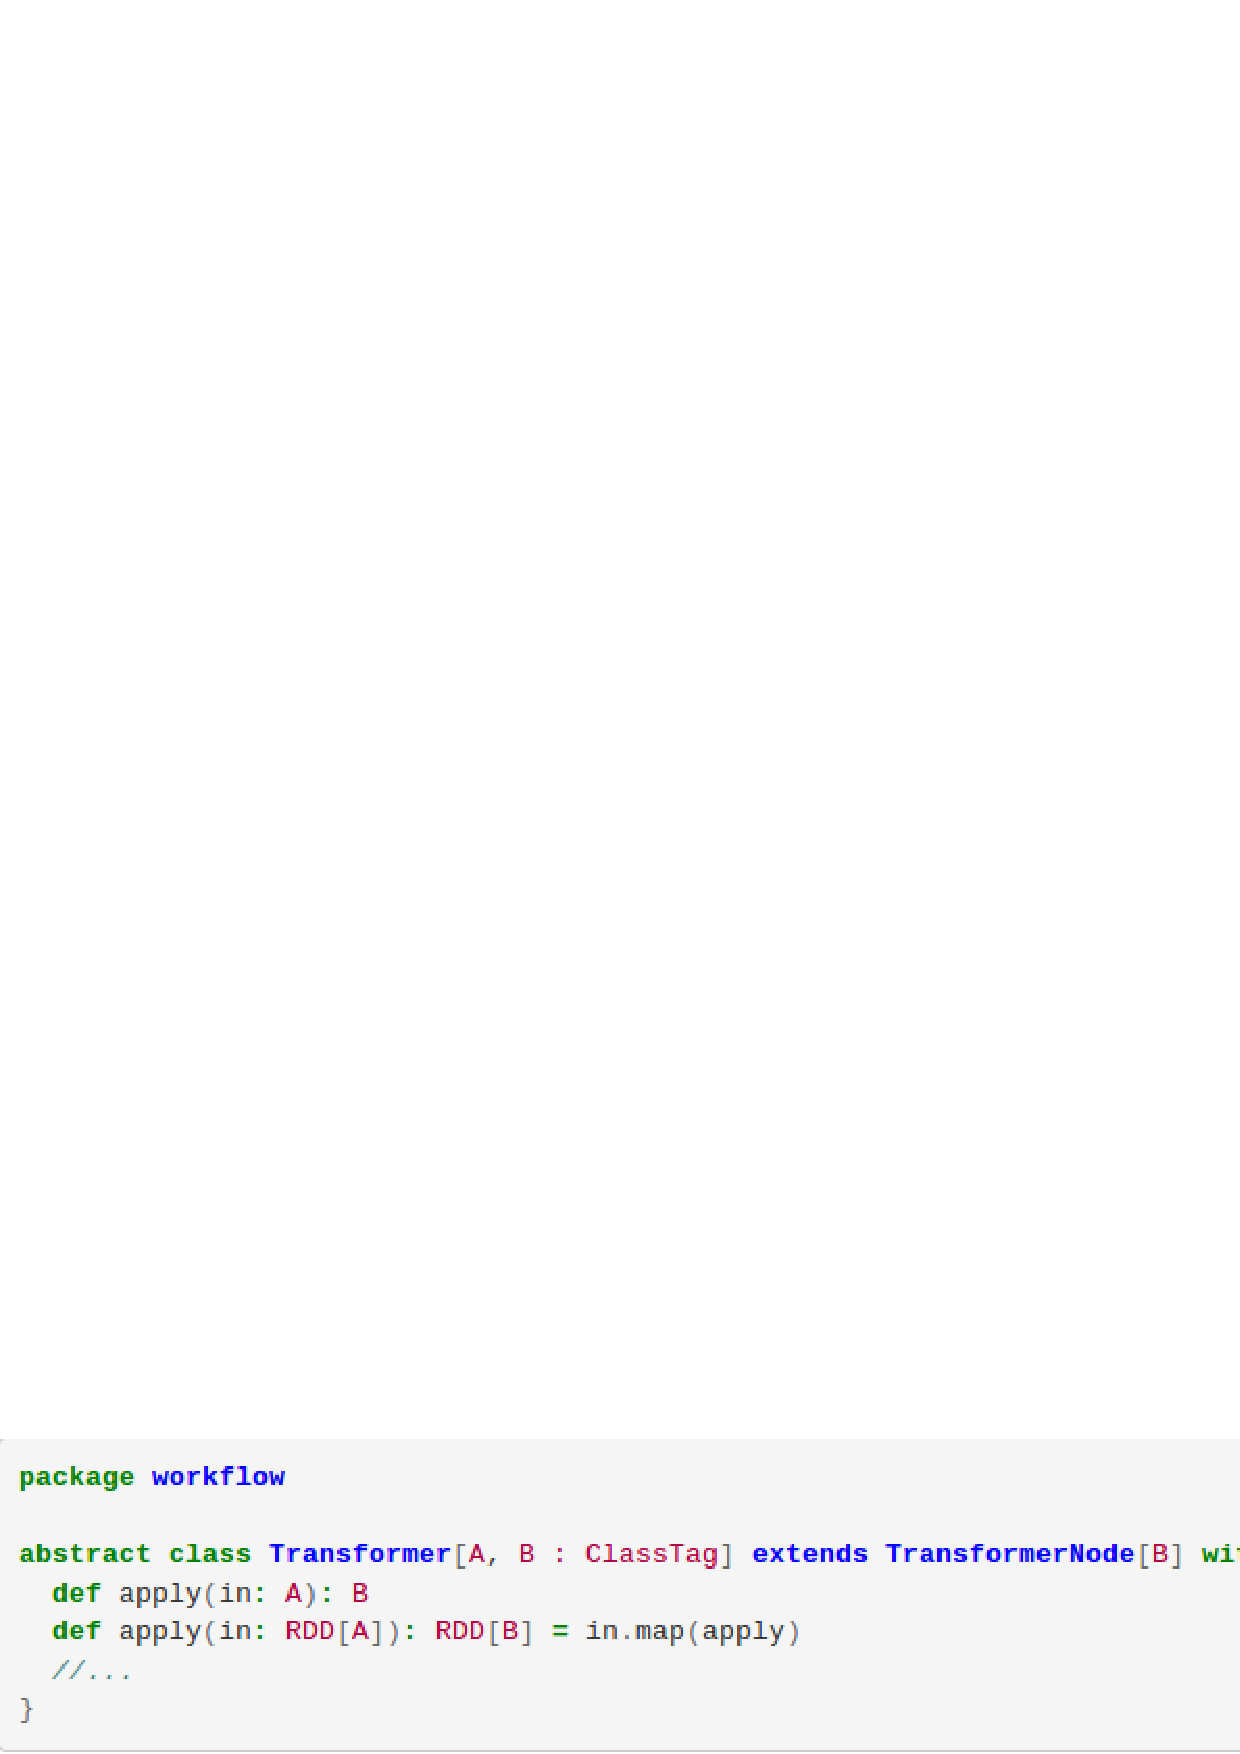
\includegraphics[width=\linewidth]{images/6}}
\caption{Transformer Class}
\label{fig:Transformer Class}
\end{figure}

While transformers are unary functions, they themselves may be
parameterized by more than just their input. To handle this case,
transformers can take additional state as constructor
parameters. Here’s a simple transformer which will add a fixed vector
from any vector it is fed as input \cite{www-keystoneml1} .

\begin{figure}[htbp]
\centering
\fbox{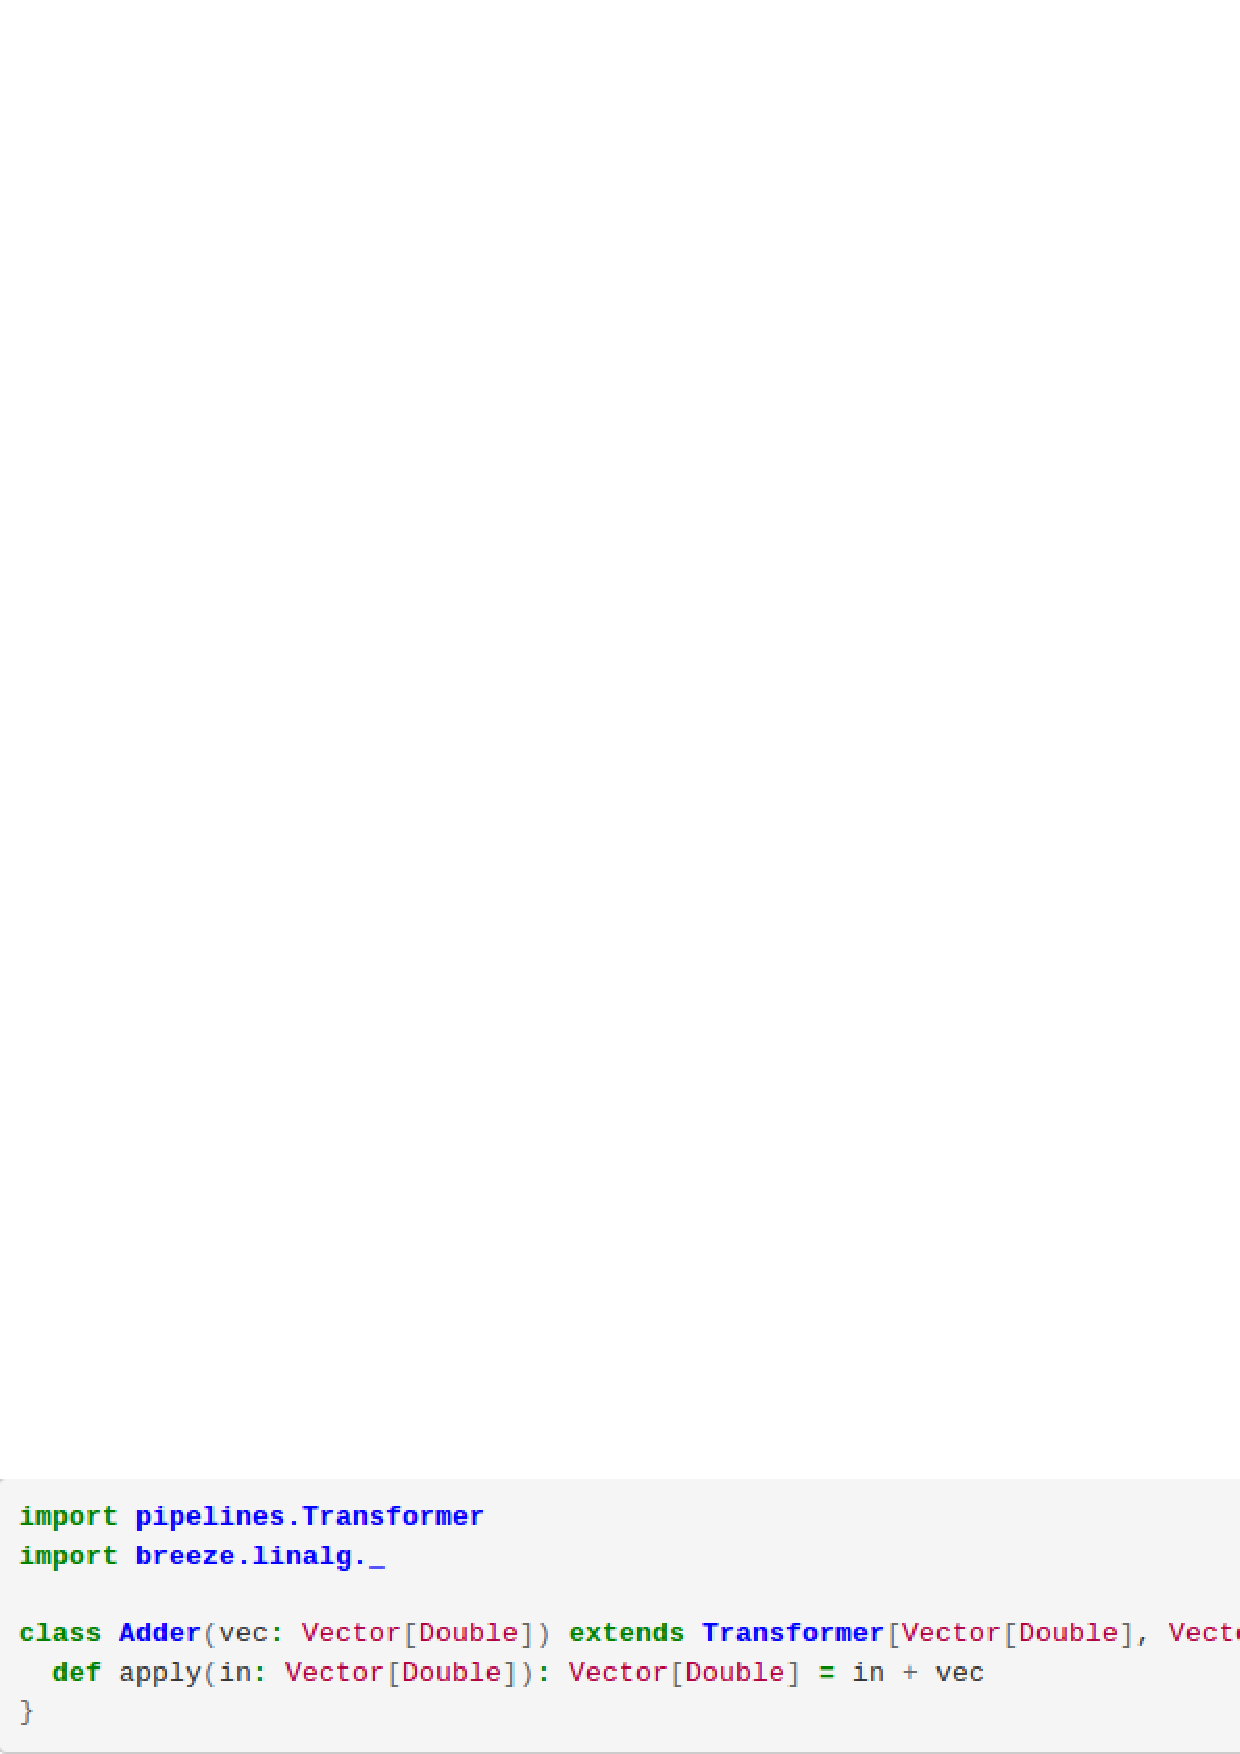
\includegraphics[width=\linewidth]{images/7}}
\caption{Transformer Class-Additional states}
\label{fig:Transformer Class-Additional states}
\end{figure}

\subsection{Estimators}

Estimators are what puts the ML in KeystoneML. An abridged Estimator
interface looks like this:

\begin{figure}[htbp]
\centering
\fbox{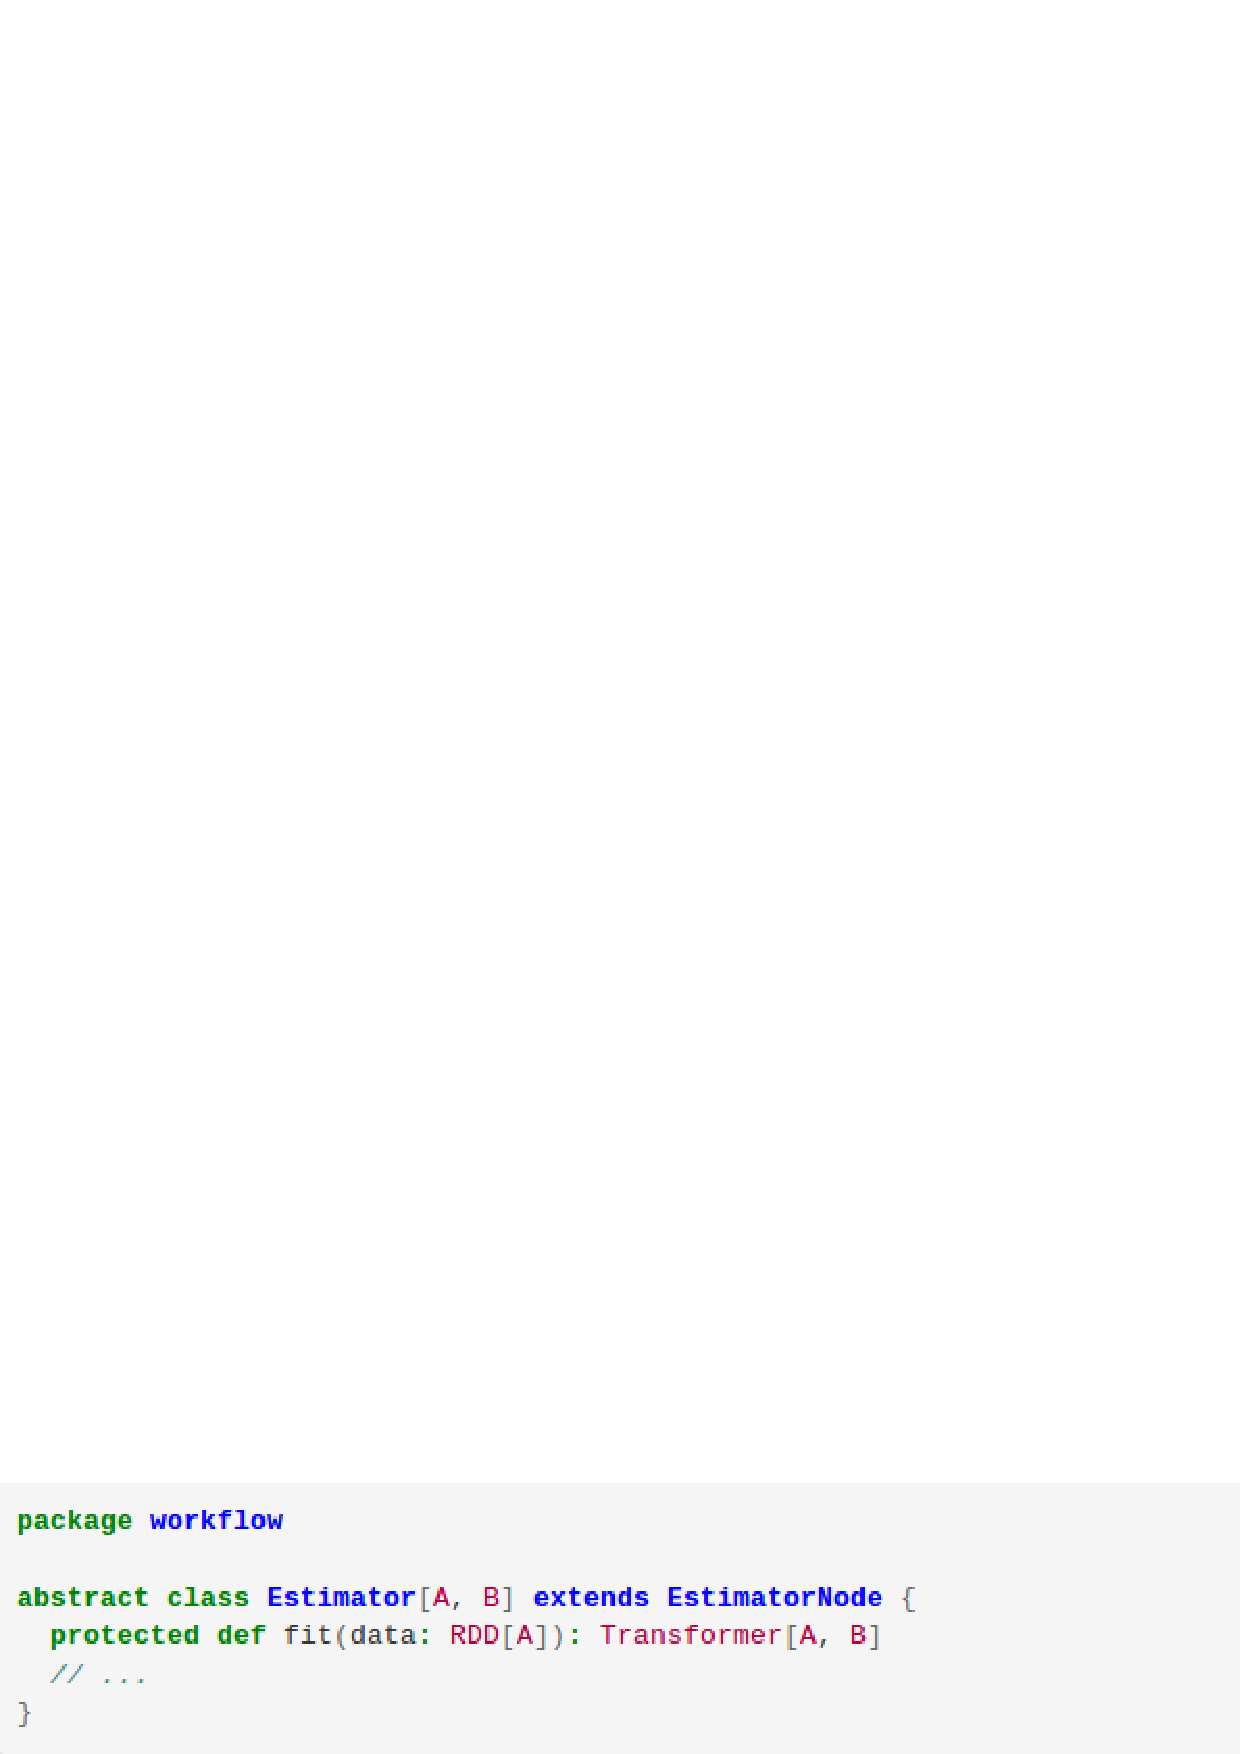
\includegraphics[width=\linewidth]{images/8}}
\caption{Estimator Interface}
\label{fig:Estimator Interface}
\end{figure}

Estimator takes in training data as an RDD to its fit() method, and
outputs a Transformer.Suppose you have a big list of vectors and you
want to subtract off the mean of each coordinate across all the
vectors (and new ones that come from the same distribution). We could
create an Estimator to do this like so.

\section{Chaining Nodes and Building Pipelines}

Pipelines are created by chaining transformers and estimators with the
andThen methods. Going back to a different part of the Transformer
interface:

Ignoring the implementation, andThen allows you to take a pipeline and
add another onto it, yielding a new Pipeline[A,C] which works by first
applying the first pipeline (A => B) and then applying the next
pipeline (B => C).

This is where type safety comes in to ensure robustness. As your
pipelines get more complicated, you may end up trying to chain
together nodes that are incompatible, but the compiler won’t let
you. This is powerful, because it means that if your pipeline
compiles, it is more likely to work when you go to run it at scale \cite{www-keystoneml} .

Estimators can be chained onto transformers via the andThen
(estimator, data) or andThen (labelEstimator, data, labels)
methods. The latter makes sense if you’re training a supervised
learning model which needs ground truth training labels. Suppose you
want to chain together a pipeline which takes a raw image, converts it
to grayscale, and then fits a linear model on the pixel space, and
returns the most likely class according to the linear model \cite{www-keystoneml} .

\section{Why KeystoneML?}

KeystoneML makes constructing even complicated machine learning
pipelines easy. Here’s an example text categorization pipeline which
creates bigram features and creates a Naive Bayes model based on the
100,000 most common features \cite{www-keystoneml1} .

\begin{figure}[htbp]
\centering
\fbox{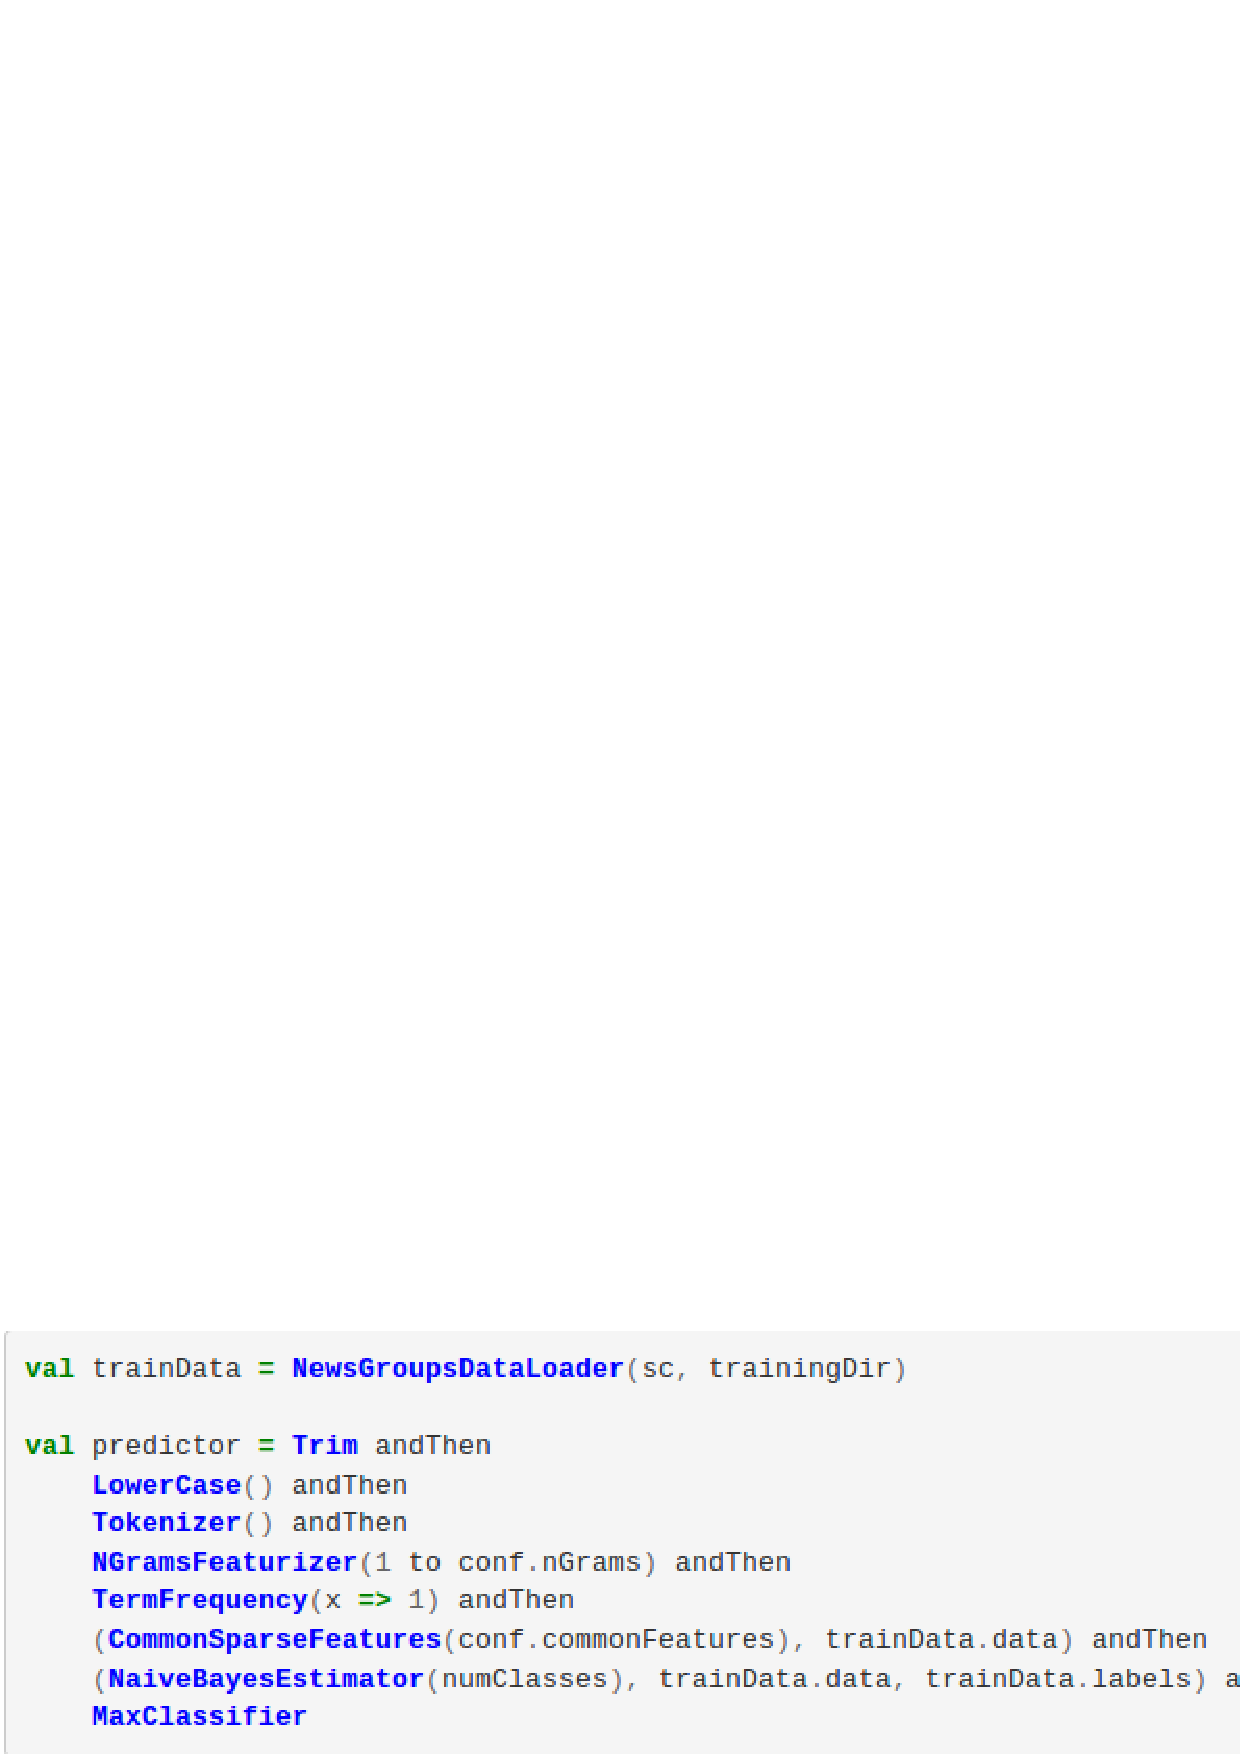
\includegraphics[width=\linewidth]{images/1}}
\caption{Code for Naive Bayes model}
\label{fig:Code for Naive Bayes model}
\end{figure}


Parallelization of the pipeline fitting
process is handled automatically and pipeline nodes are designed to
scale horizontally. Once the pipeline has been defined you can apply
it to test data and evaluate its effectiveness \cite{www-keystoneml} .

\begin{figure}[htbp]
\centering
\fbox{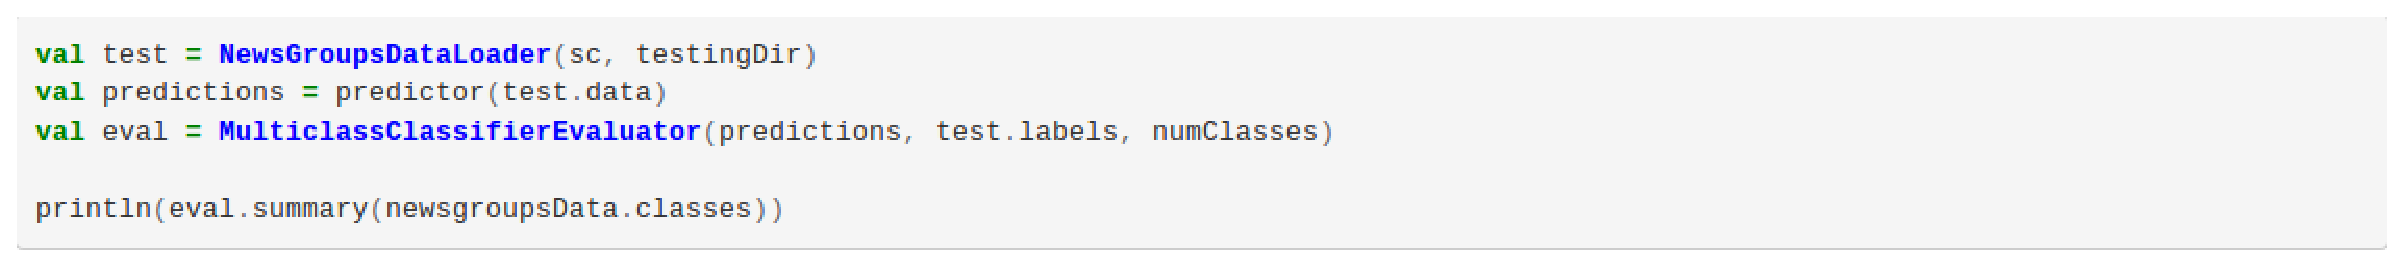
\includegraphics[width=\linewidth]{images/2}}
\caption{Code for testing the data for effectiveness}
\label{fig:Code for testing the data for effectiveness}
\end{figure}


The result of this code is as follows:

\begin{figure}[htbp]
\centering
\fbox{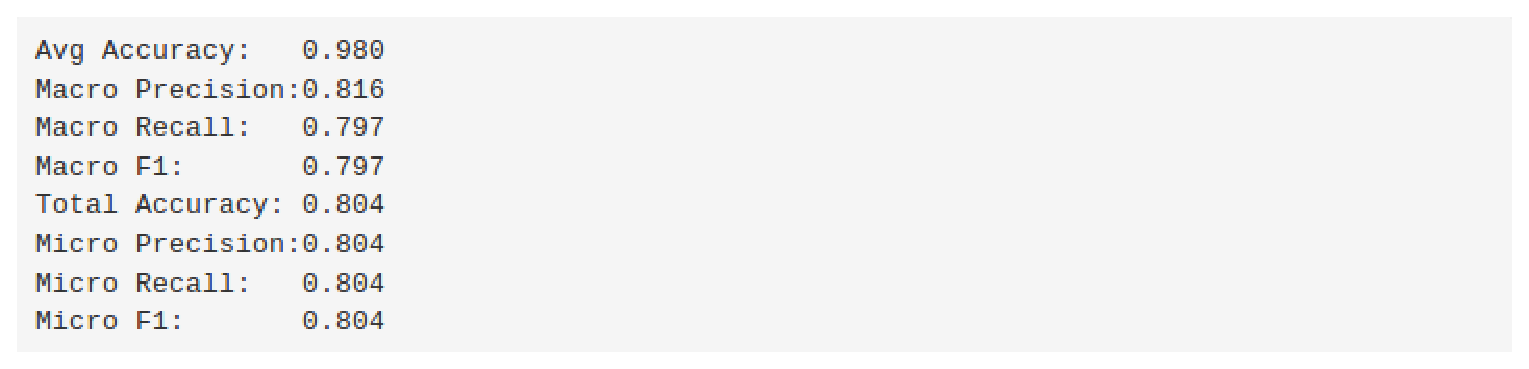
\includegraphics[width=\linewidth]{images/3}}
\caption{Output for the above code}
\label{fig:Output for the above code}
\end{figure}

This relatively simple pipeline predicts the right document category
over 80 percent of the time on the test set. KeystoneML works with
much more than just text. KeystoneML is alpha software, in a very
early public release (v0.2). The project is still very young, but it
has reached a point where it is viable for general use.

\section{Linking}

KeystoneML is available from Maven Central. It can be used in our
applications by adding the following lines to the SBT project
definition:

libraryDependencies += "edu.berkeley.cs.amplab" % "keystoneml_2.10" % "0.3.0"



\section{Building}

KeystineML is available on GitHub.

\$ git clone https://github.com/amplab/keystone.git

Once downloaded, KeystoneML can be built using the following commands:

\$ cd keystone

\$ git checkout branch-v0.3

\$ sbt/sbt assembly

\$ make

You can then run example pipelines with the included
bin/run-pipeline.sh script, or pass as an argument to spark-submit.

\section{Running an Example}

Once you’ve built KeystoneML, you can run many of the example
pipelines locally. However, to run the larger examples, you’ll want
access to a Spark cluster.

Here’s an example of running a handwriting recognition pipeline on the
popular MNIST dataset. This should be able to run on a single
machine in under a minute.

\begin{figure}[htbp]
\centering
\fbox{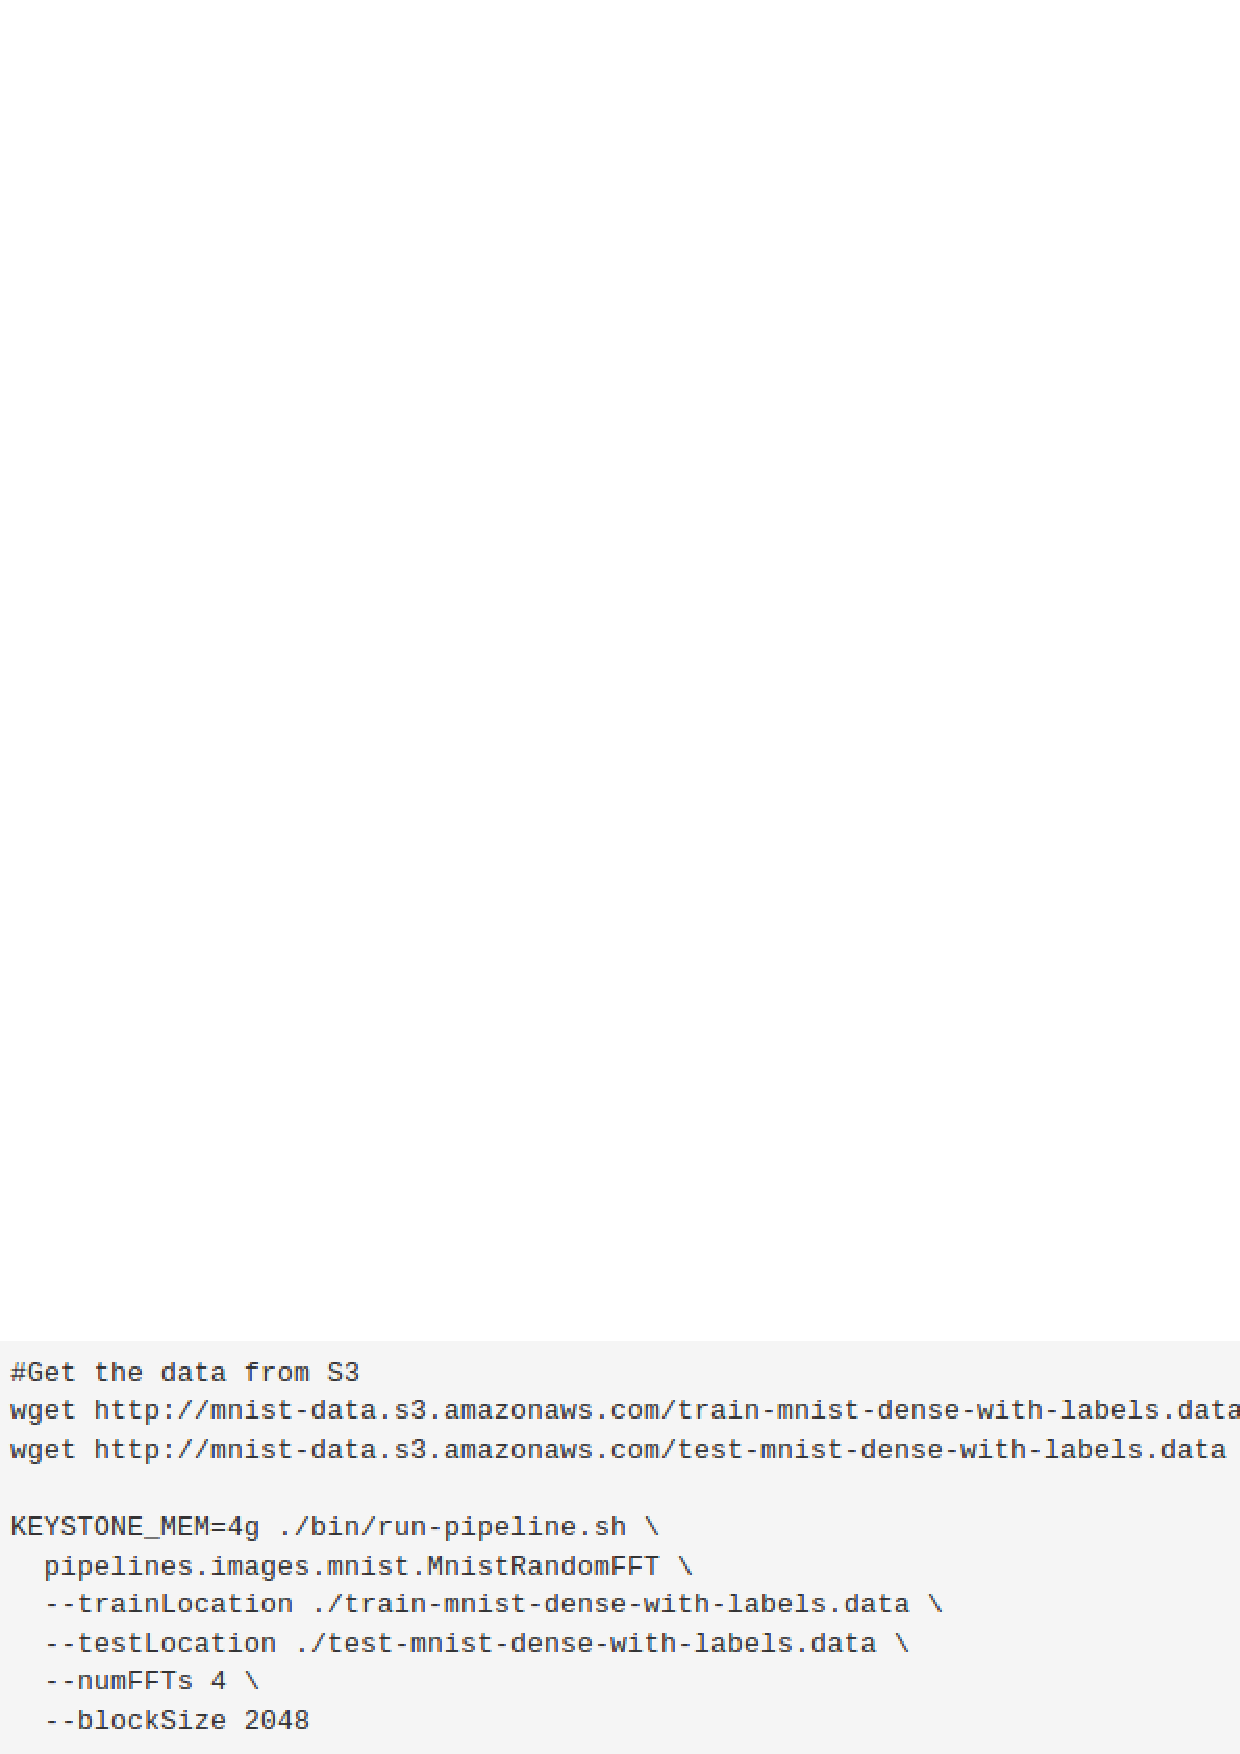
\includegraphics[width=\linewidth]{images/4}}
\caption{Example for running on a MNIST dataset}
\label{fig:Example for running on a MNIST dataset}
\end{figure}

To run on a cluster, it is recommend using the spark-ec2 to launch a
cluster and provision with correct versions of BLAS and native C
libraries used by KeystoneML.

More scripts have been provided to set up a well-configured cluster
automatically in bin/pipelines-ec2.sh.


\section{Conclusion}

One of the main features of KeystoneML is the example pipelines and
nodes it provides out of the box. These are designed to illustrate
end-to-end real world pipelines in computer vision, speech
recognition, and natural language processing. KeystoneML also provides
several utilities for evaluating models once they’ve been
trained. Computing metrics like precision, recall, and accuracy on a
test set. Metrics are currently calculated for Binary Classification,
Multiclass Classification, and Multilabel Classification, with more on
the way \cite{www-keystoneml} .


% Bibliography

\bibliography{references}

\end{document}
